\section{Diskussion}
\label{sec:Diskussion}
Der für die Messung im 30-1000 milli Bar bestimmte Wert der Verdampfungswärme $L$
\begin{equation*}
    L = (39290,2052\pm 307,0932)\unit{\joule\per\mol}
\end{equation*}
weicht im vergleich mit dem Literaturwert der Verdampfungswärme $L_{ref}$ \cite{Chem} von Wasser bei $\SI{100}{\celsius}$
\begin{equation*}
    L_{ref} = \SI{40,7}{\kilo\joule\per\mol}
\end{equation*}
ergibt sich eine Abweichung von ca. $2,71\%$.\\
Die zur Messreihe im 1-15 Bar Bereich berechneten $L$, ergeben in \autoref{fig:LAdd} keine sinnvollen Plot und sind daher stark Fehlerbehaftet.
Dies kann an der Messaperatur liegen, da diese bereits bei $\SI{108}{\celsius}$ eine Wert von $\SI{1}{\bar}$ erricht hatte und dieser erst bei
ca. $\SI{120}{\celsius}$ auftreten sollte. Außerdem sind systematische Fehler beim Ablesen nicht auszuschließen.
Zudem hängen die $L$ vom Differentialquotienten $\frac{dp}{dT}$ ab, welcher mehrere ungenaue,
durch eine Ausgleichsrechnung bestimmte, Konstanten beinhaltet.
\section{Anhang}
\label{sec:Anhang}
\begin{figure}[H]
    \centering
    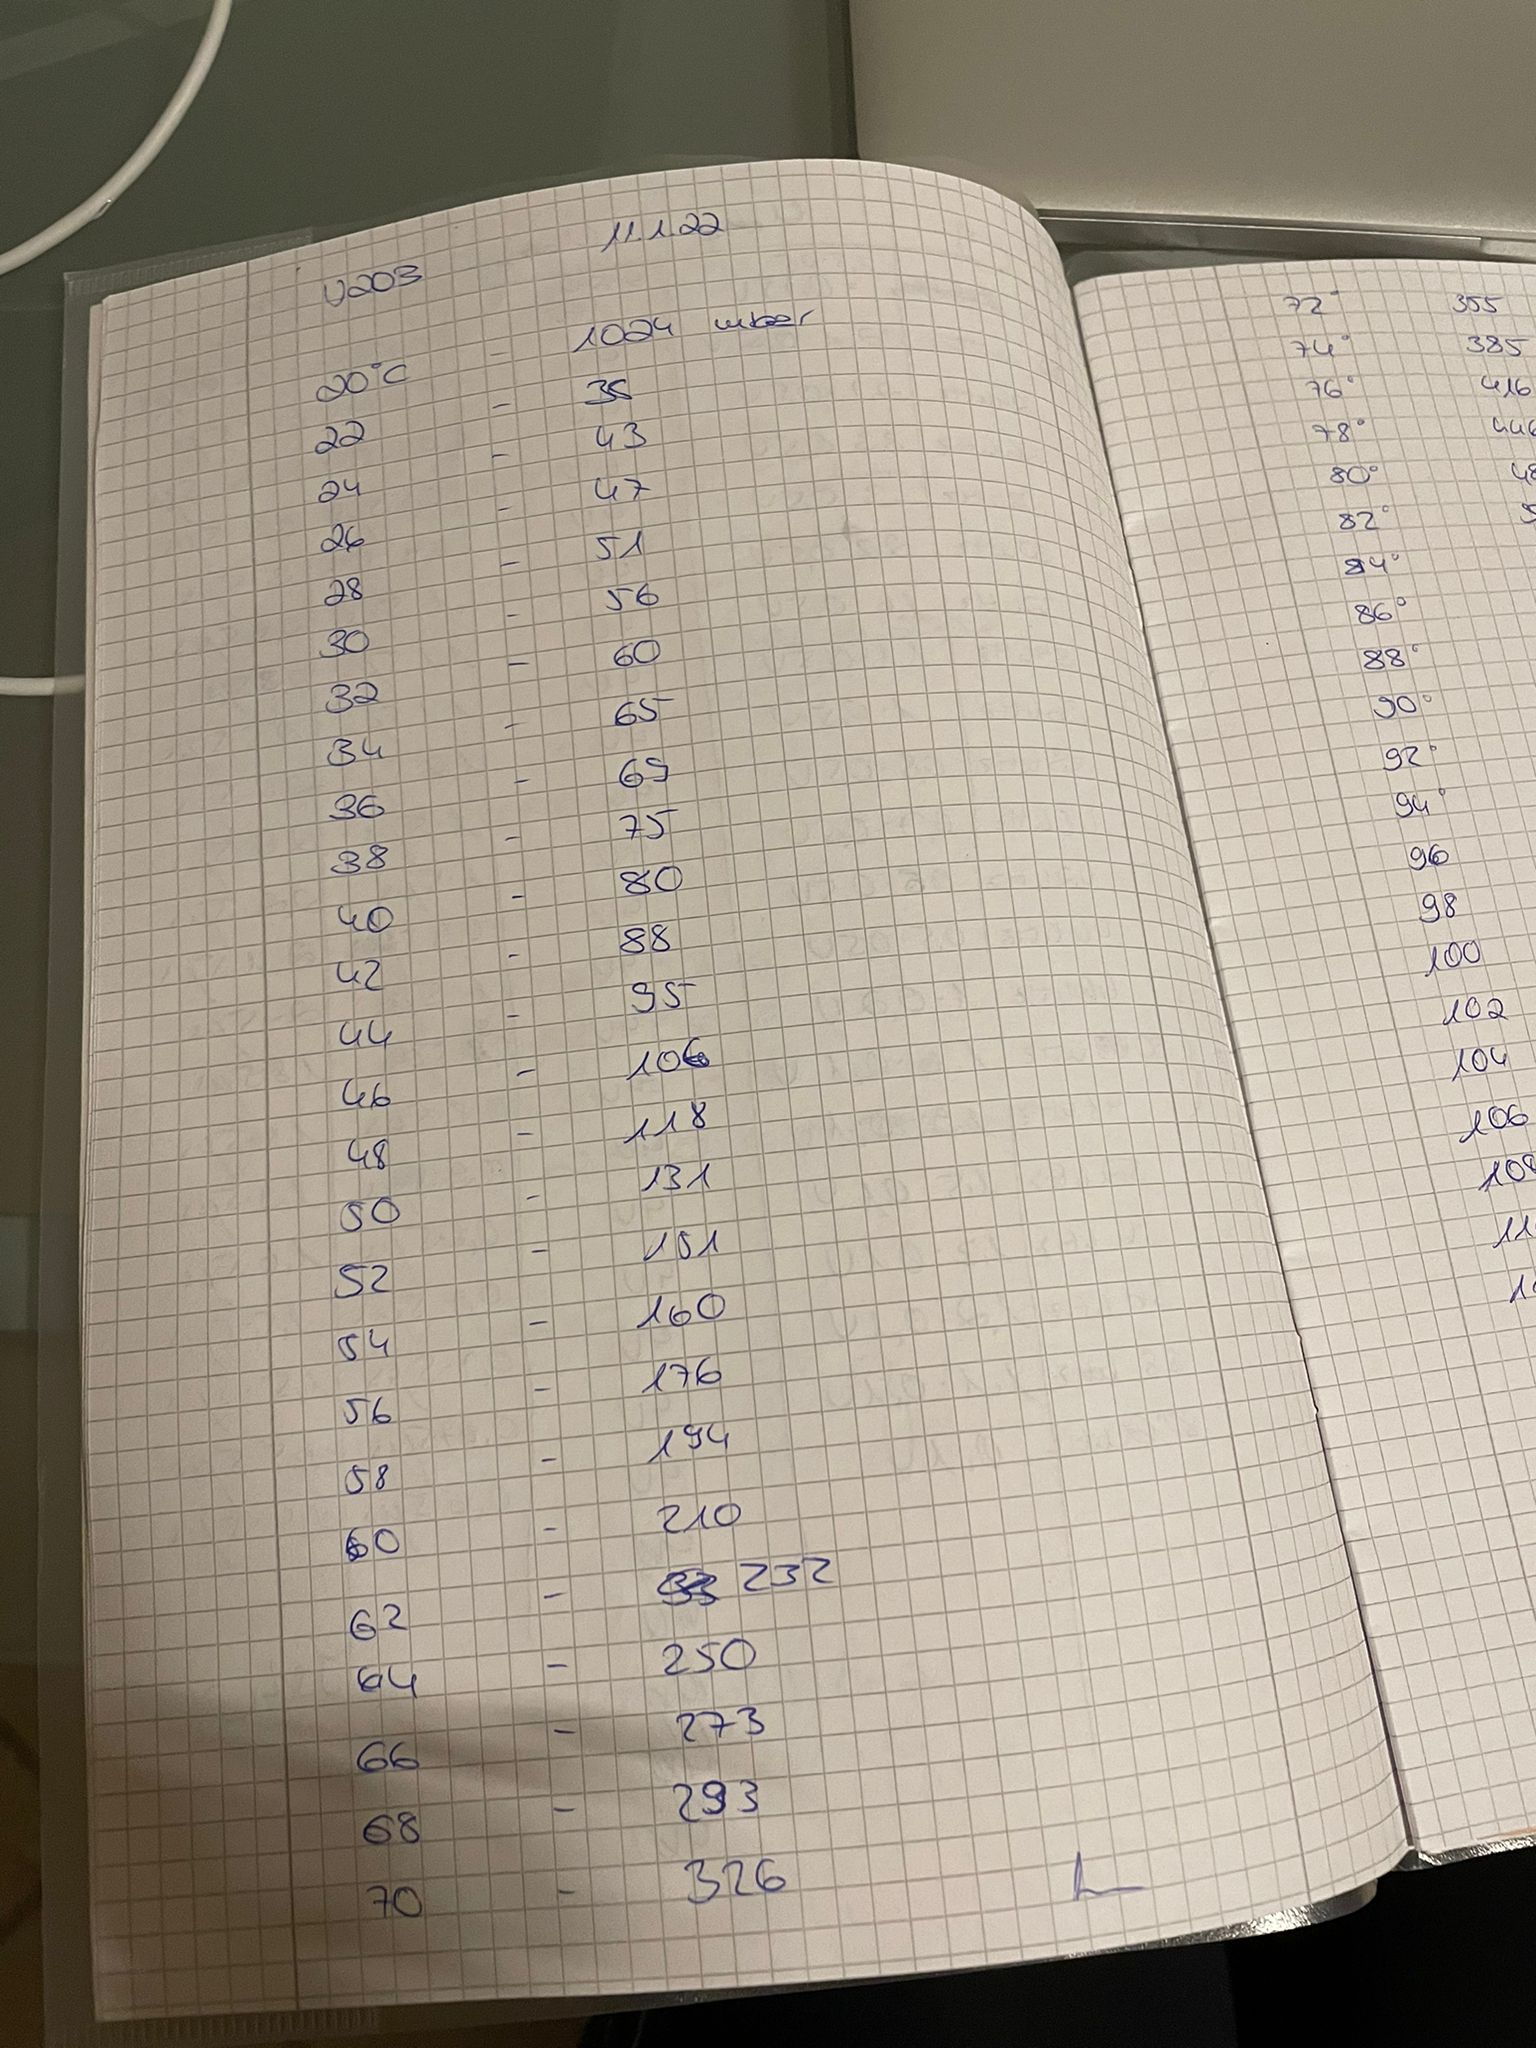
\includegraphics[scale=0.2]{content/OrgDat1.png}
    \caption{Die Originaldaten.}
    \label{fig:OrgDat1}
\end{figure}
\begin{figure}[H]
    \centering
    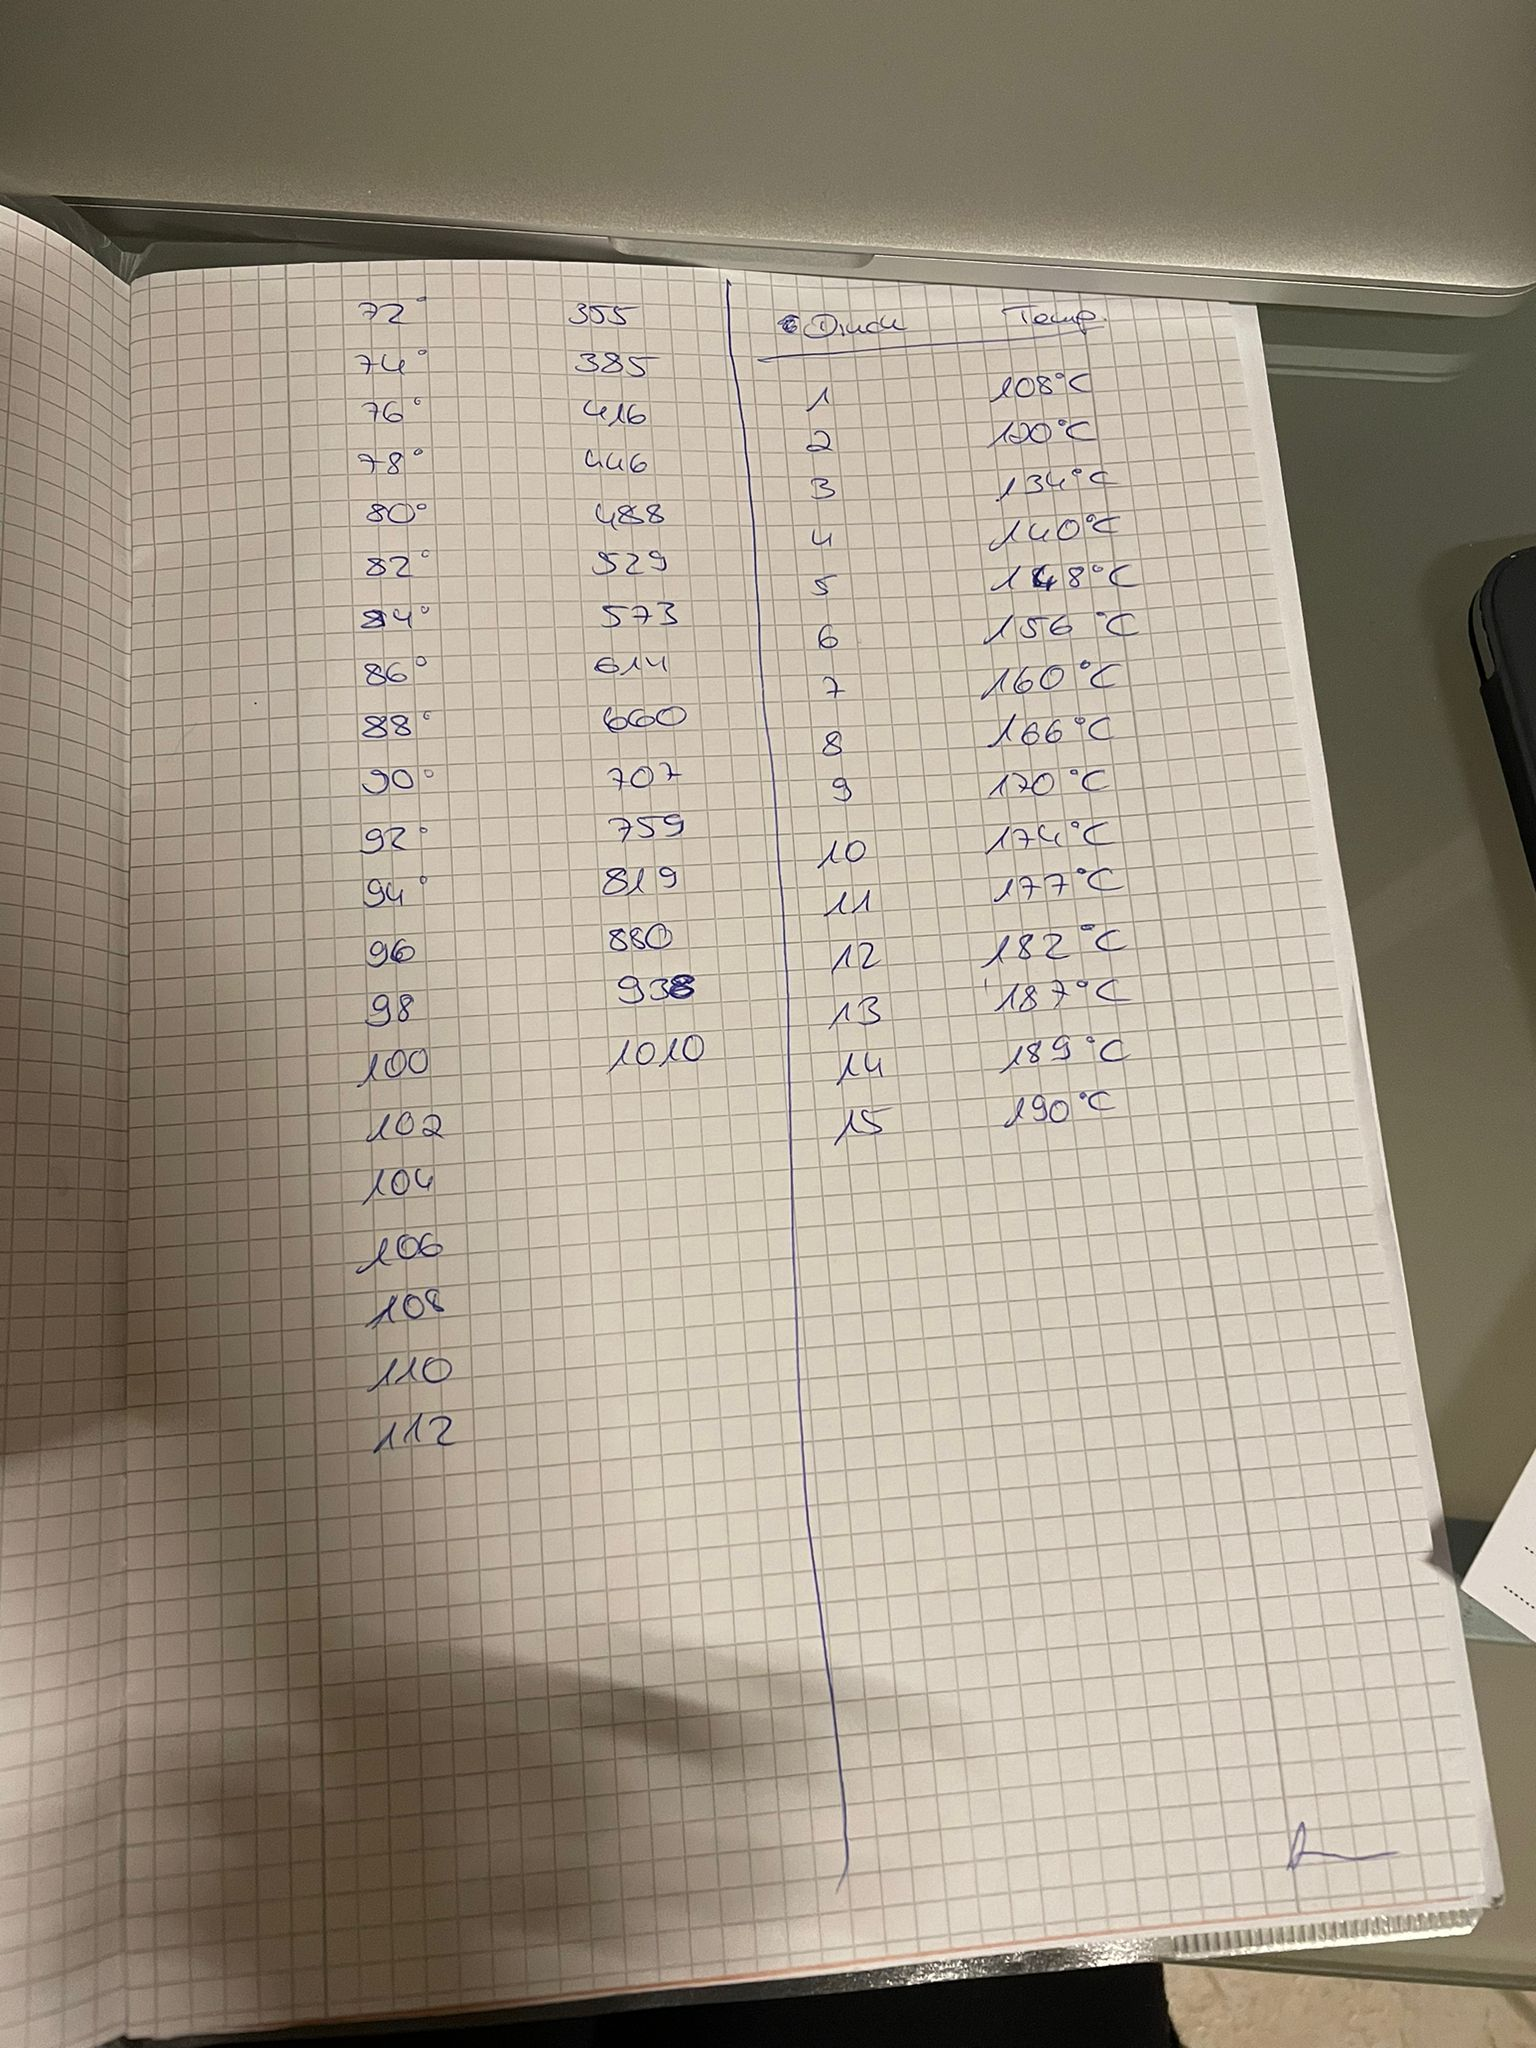
\includegraphics[scale=0.2]{content/OrgDat2.png}
    \caption{Die Originaldaten.}
    \label{fig:OrgDat2}
\end{figure}
